
\subsubsection{Alternatives to Distributed machine learning}
Even though the most popular solution to increasing computation power for Machine
learning is currently distributing the workload over a large amount of machines,
there are other more traditional ways to increase computation power. These ways
include the use of Application Specific Integrated Circuits and special multi-core
computer architectures.

\paragraph{ASICs}
The idea of using ASICs in highly specialized tasks is not a new idea
to machine learning. In recent times the demand for such chips has risen massively\cite{Metz18}.
For example, for applications like Bitcoin mining, ASICs have a massive competitive
advantage over GPUs and CPUs, rendering them essentially useless. The main reason
that the expectations of ASICs are very high when looking at Machine
Learning is the fact that most of the work in most areas are matrix multiplications,
an area in which some ASICs excel.

Google took this idea of ASICs and have created their own Tensor Processing Unit (TPU)\cite{Sato17},
which, as the name suggests, is an ASIC that specializes in calculations that
use tensors. This works well together with their TensorFlow library, which is one
of the most popular Neural Network Libraries around at the moment. The architecture of
such a chip can be seen in Figure \ref{TPU_Architecture}.

\begin{figure}
  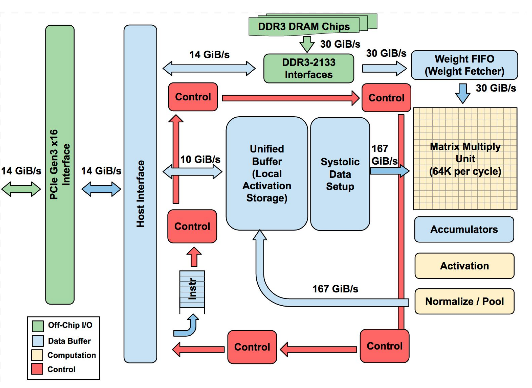
\includegraphics[width=\textwidth]{TPU_Architecture.png}
  \caption{Google TPU Architecture\cite{Joup17}}
  \label{TPU_Architecture}
\end{figure}

The most important aspect of the TPU is the Matrix Multiply unit that is positioned
on the right of the diagram. As can be seen, the TPU uses a PCIe bus to communicate
with a server so it is not a stand-alone unit ()which is useful as it can then also
be used in a distributed setting).

The performance improvement of the TPU over regular CPU/GPU combinations is not only
the increased processing power, but also the efficiency, which is important
for big companies that want want to minimize their energy costs. In Figure \ref{TPU_Relative_Performance},
it can be seen that the performance/watt of a TPU relative to GPUs and CPUs is many times higher,
up to nearly 200x the performance/watt.

\begin{figure}
  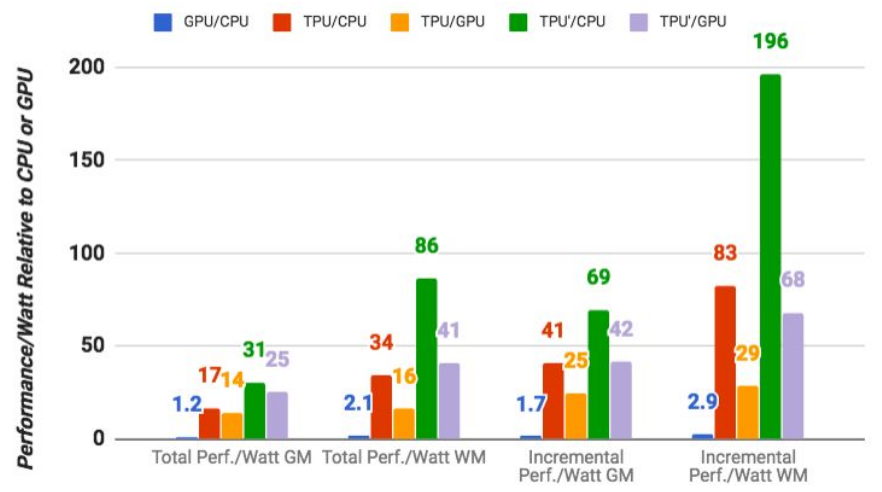
\includegraphics[width=\textwidth]{TPU_Relative_Performance.png}
  \caption{TPU performance, relative to CPU and GPU, the total performance includes server power costs. GM and WM are geometric and weighted means respectively \cite{Joup17}}
  \label{TPU_Relative_Performance}
\end{figure}

Other than the power efficiency, the total processing power of a TPU is also a lot higher
than a GPU or CPU. This is illustrated in Figure \ref{TPU_Performance} that shows that the 
power consumption of a TPU is a lot lower than that of a a CPU or GPU in most cases.

\begin{figure}
  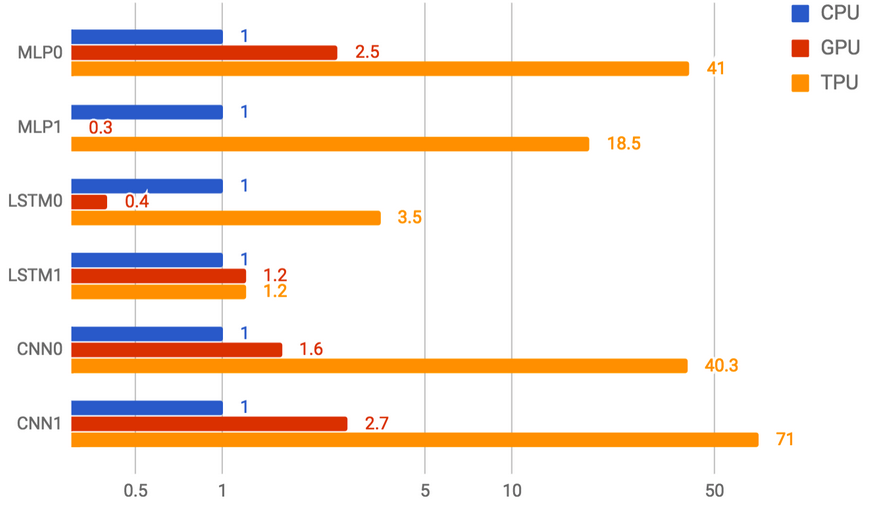
\includegraphics[width=\textwidth]{TPU_Performance.png}
  \caption{TPU performance on 6 common machine learning tasks\cite{Sato17}}
  \label{TPU_Performance}
\end{figure}


\paragraph{Computer architectures}
Other than using ASICs in order to increase the amount of work a computer can do,
a different architecture can also be used that is designed to increase the amount
of usable cores on a computer massively. Such an architecture exists in the form
of the Epiphany architecture. The Epiphany architecture is a Multiple Instruction,
Multiple Data (MIMD) architecture that uses an array of processors, that all use the
same memory to speed up execution of floating point operations\cite{Olof16}.

The newest chip of the major manufacturer Adapteva is the Epihpany V, which uses
1024 cores on a single chip\cite{Olof16}. Although Adapteva has not publicsed the power consumption of the Epiphany V yet,
it has released numbers boasting a power usage of only 2 watt\cite{Adap}.

Using multiple processors to process a single dataset is not a new idea in computer
Science. For this purpose MPI was developed to simplify the distribution of work,
usually over a cluster of workers. The same framework can also be adapted to the
Epiphany chips as was demonstrated by Richie et al. in their paper. They found that
the RISC chips were able to perform extremely fast matrix operations until their on board
memory was filled\cite{Rich15}. In Figure \ref{Epiphany_MPI} it can be seen that performance increases
until the matrix no longer fits in memory.

\begin{figure}
  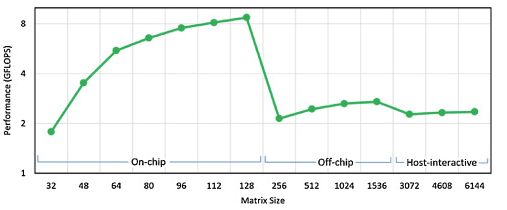
\includegraphics[width=\textwidth]{Epiphany_MPI.png}
  \caption{Epiphany chip performance with different matrix sizes\cite{Rich15}.}
  \label{Epiphany_MPI}
\end{figure}

\paragraph{Future relevance}
As can be seen with the examples above, there are many different ways to get the processing
power needed to use large-scale Machine Learning. These techniques focus both on
power efficiency as well as on computational power. However, it must be noted
that due to the benefits of space and power consumption that distributed systems can offer,
these are generally preferred above these non-distributed alternatives. However, all of these
techniques described above can be used in a distributed setting without major performance degradations.
This makes them a good choice for future applications, as they can use the benefits of both optimized hardware and distributed systems.
